\documentclass{article}
\title{Tendermint Evaluation}
\author{Simone Petruzzi-1811872 Domenico Tersigni-1817502}
\date{August 2023}
\usepackage[margin=1.5in]{geometry} % Adjust the values as per your requirements
\usepackage{amssymb}
\usepackage{amsfonts}
\usepackage{amsmath}
\usepackage{graphicx}
\graphicspath{ {./images/} }
\usepackage{xcolor}
\usepackage{listings}
\lstdefinestyle{bashstyle}{
    language=Bash,
    basicstyle=\ttfamily,
    keywordstyle=\color{blue},
    commentstyle=\color{green!40!black},
    numbers=left,
    numberstyle=\tiny,
    numbersep=5pt,
    frame=single,
    breaklines=true,
    breakatwhitespace=true,
    tabsize=4
}

\begin{document}
   \maketitle
   \section{Introduction}
   Consensus has a very important role in the context of State Machine Replication (SMR). The key idea for this kind of approach is that service replicas start in the exact same initial state, then executing requests in the same order. In this sense Consensus plays a fundamental role ensuring that all replicas receive transactions in the same order.
   \newline
   \newline
   Here we are considering not data center context (traditional architecture for deployment of SMR based systems), with the success of cyptocurrencies and blockchain systems we have different requirements. Indeed in this kind of context we have that nodes are not all connected to each others like in the data center context, but only to a subset of nodes of the network. Communication between nodes is achieved by gossip-base peer-to-peer protocols.
   \subsection{Model}
   We consider a system of processes that communicate by exchanging messages. Processes can be correct or faulty (we consider the Byzantine case in which a process can act maliciously inside the network: for example by forging messages or avoiding to replay), each of it having some amount of voting power (it can also be 0). As we said previously we don't consider processes as part of a single administrative domain, conversely we assume that each process is able to exchange messages only with a subset of processes of the entire network. Communication between processes of the same domain happens through gossip protocol. We structure network communication through a modified version of the partially synchronized system model, in which we have an upper time bound $\Delta$ such that it is the maximum time we can wait and a time instant GST (Global Stabilization Time), after that all the communication among corrects is reliable. \\
   Termination of the algorithm is guaranteed within a bounded duration after GST. Processes are equipped with a clock and they can measure local timeouts. Spoofing is not possible due to public-key cryptography (all messages contains digital signatures).
   \subsection{State Machine replication}
   Key idea of this approach is to guarantee that all replicas start at the same state and then proceed in the same order processing requests:
   \begin{itemize}
   	\item Replica coordination: all non-faulty replicas receive and process the same sequence of requests.
   \end{itemize}
   there is also an additional requirement that needs to be ensured: only the requests sent by clients must be executed.\\
   In Tendermint is the service that is replicated that takes care of accepting or rejecting transactions. When a request arrives, the Tendermint process will ask the service if the request is valid, and only valid requests can be processed.
   \subsection{Consensus}
   Tendermint solves the state machine replication problem by sequentially executing consensus instances to agree on each block of transaction that are executed by the service being replicated. This problem is defined in terms of an agreement, a termination and a validity property.
   \begin{itemize}
   	\item \textbf{Agreement}: No two correct processes decide on different values.
	\item \textbf{Termination}: All correct processes eventually decide on a value.
	\item \textbf{Validity}: A decided value is valid, i.e., it satisfies the predefined predicate denoted valid().
   \end{itemize}
   \newpage
   \section{Tendermint consensus algorithm}
   We assume that there is a gossip-based protocol for disseminating messages, and every process stores messages in a local message log for every process. The algorithm is presented as a set of upon rules that are triggered once the message log contains messages such that the corresponding condition evaluates to true. \\
   The algorithm proceeds in rounds, each of it having a dedicated proposer. Processes are all aware of the rounds by simply processing the $propose(h,round)$ function, that returns the proposer for the $round$ in the consensus instance $h$. In each round of consensus, one validator is selected as the proposer through a weighted round robin function, where processes are rotated proportional to their voting power.\\ \\
	Processes in Tendermint exchange three types of messages: PROPOSAL, PREVOTE, PRECOMMIT. Thus Tendermint, requires two voting steps (three communication exchanges of messages in total). The PROPOSAL message is the only carrying the value $v$ (in this context a block of transactions) and a value id, PREVOTE and PRECOMMIT carry only the value id. A correct process decides a value $v$ after having received $2f+1$ voting power equivalent PRECOMMIT messages for it. In order to send PRECOMMIT for some messge $v$ in a round $r$ a process must wait for the PROPOSAL and $2f+1$ of the corresponding PREVOTE messages in the round $r$. Otherwise it sends PRECOMMIT message with a special $nil$ value (ensuring that corrects can PRECOMMIT only a single value in a round). Since proposers may be faulty , the proposed value is treated by corrects like a suggestion, and corrects tell each others if they accepted the PROPOSAL for a certain value by sending PREVOTE message for it. Otherwise like for the PRECOMMIT message, it sends PREVOTE message with a $nil$ value. \\ \\
	Every process mantain the following variables: $step$, $lockedValue$, $lockedRound$, $validValue$ and $validRound$. The $step$ denotes the stage of the algorithm execution in the current round. $lockedValue$ holds the latest value sent with a PRECOMMIT message for a specific round number, and $lockedRound$ is the last round with a non-$nil$ PRECOMMIT message. A correct process locks a value $v$ in round r by setting $lockedValue$ = $v$ and $lockedRound$ = r before sending a PRECOMMIT message for id(v). To make a decision, a correct process needs 2f + 1 PRECOMMIT messages for id(v), meaning a possible decision value is locked by at least f + 1 voting power equivalent of correct processes. Thus, any value v receiving PROPOSAL and 2f + 1 corresponding PREVOTE messages in round r is a possible decision value. $validValue$ stores the most recent possible decision value, and $validRound$ is the last round it was updated. Additionally, each process stores its current consensus instance ($h_p$ or height in Tendermint) and the current round number ($round_p$) attached to every message. Finally, a process maintains an array of decisions, $decision_p$, for each consensus instance. \\ \\	
	Each round starts with a proposer using a PROPOSAL message to suggest a value. In the first round of each height, the proposer can freely choose the suggested value. A correct process gets a proposal value using the external function $getValue()$, ensuring it's valid. In subsequent rounds, a correct proposer only suggests a new value if $validValue$ is $nil$. Otherwise, $validValue$ is proposed. The PROPOSAL message includes $validRound$ to inform others of the last round where $validValue$ was considered a possible decision. If a correct process $p$ sends $validValue$ with $validRound$ in the PROPOSAL, it means $p$ received PROPOSAL and the corresponding $2f + 1$ PREVOTE messages for $validValue$ in $validRound$. When a correct process sends a PROPOSAL message with $validValue$ ($validRound > -1$) at time t $>$ GST, gossip communication ensures all correct processes receive the PROPOSAL and PREVOTE messages before $t + \Delta$. Thus, they can verify the suggested value's correctness, supported by the PROPOSAL and 2f + 1 equivalent voting power PREVOTE messages. \\ \\
	A correct process $p$ accepts a proposal for value $v$ (i,e. sends PREVOTE for $id(v)$) if an external valid function approves $v$, and if $p$ has not locked any value ($lockedRound = -1 $) or has locked value $v$ ($lockedValue = v$). If the proposed pair is (v, vr $\geq$ 0), and a correct process p has already locked a value, it will accept v if it's a more recent possible decision value ($v_r > lockedRound_p$) or if $lockedValue = v$. Otherwise, a correct process rejects the proposal by sending a PREVOTE message with a nil value. Additionally, a correct process sends a PREVOTE message with a nil value if the $timeoutPropose$ has expired (triggered when a correct process starts a new round) and the process hasn't sent a PREVOTE message in the current round yet.\\ \\
	When a correct accepts a proposal for a value $v$ by sending a PRECOMMIT message with $id(v)$ if it receives a PROPOSAL message for $v$ along with 2f + 1 PREVOTE messages for $id(v$). Otherwise, it sends a PRECOMMIT message with a nil value. In the event that a correct process hasn't sent a PRECOMMIT message in the current round and the $timeoutPrevote$ has expired, it will also send a PRECOMMIT message with a nil value.To make a decision, a correct process requires receiving a PROPOSAL message for a value $v$ in some round $r$ and requires receiving also 2f + 1 PRECOMMIT messages referencing id(v). To prevent the algorithm from becoming stuck indefinitely,it is used $timeoutPrecommit$, which triggers after a process receives any set of 2f + 1 PRECOMMIT messages for the current round. If the $timeoutPrecommit$ expires and a process hasn't made a decision yet, it initiates the next round. Upon reaching a decision, a correct process $P$ initiates the next consensus instance for the subsequent height. The Gossip communication property ensures that the PROPOSAL and 2f + 1 PREVOTE messages that led $p$ to make a decision will eventually be received by all correct processes, facilitating their own decision-making process.
	\subsection{Termination mechanism}
	\newpage
	\section{Tendermint}
	Now that we talked about the consensus algorithm, let's talk about Tendermint in general. Tendermint is basically two things:
	\begin{itemize}
	 	\item Tendermint Core
	 	\item Application Block Chain Interface (ABCI)
	\end{itemize}
	\subsection{Tendermint Core}
	Tendermint Core is the actual consensus engine, and protocol. It works like practical Byzantine fault tolerant, with rotating leaders. It tolerates up to $\frac{1}{3}$ nodes failing. This is a proof of stake (PoS) protocol, thus there is no mining and validators as previously said, may not have equal voting power.
	\subsection{ABCI}
	This is the interface that allows your app to communicate with Tendermint Core and ensures that the app is properly replicated across all correct nodes in the network. The application must be deterministic. It must implement few methods:
	\paragraph{CheckTx}
	The check transaction method is responsible for checking that a transaction is properly formatted, has correct signature and more in general that it conforms to the protocol. This is the only method that receives transactions before consensus has been run on them. Thus this method should not modify the application state at all.
	\paragraph{DeliverTx}
	The deliver transaction is the method that takes a transaction and modifies the application state (eg: change account balance). This method is called for each transaction in a block and then commit is called.
	\paragraph{Commit}
	This method persist the application state and is responsible for computing the hash of the application state and returning it. This hash can lately be used to validate queries.
	\paragraph{Query}
	This method is used to query a piece of the application state (eg. balance of a single account). Ideally it should include some kind of proof that the piece of the application state it is returning, belongs to a certain application state within an application hash. \\
	\begin{figure}[htbp]
    \centering
    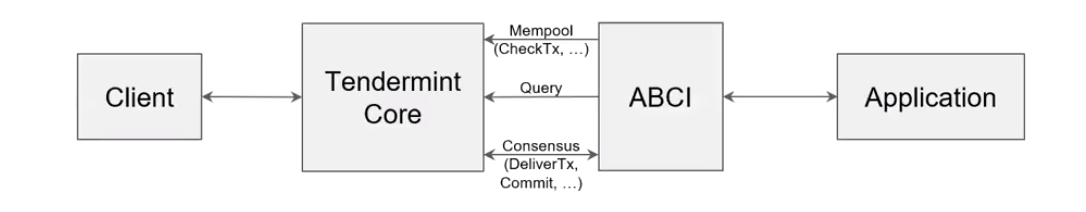
\includegraphics[width=1\textwidth]{im1} 
    \caption{architecture}
	\end{figure}\\
    Let'see in general, how a system based on Tendermint works. Users in the system submit transactions to a certain node, and those transactions first run into the application CheckTx method. In case the transaction don't pass the check, it will be handled by the application. If instead, the transaction is valid, it is included in the mempool, attending for being included in a block. When a validator proposes a new block, it selects some transactions from its mempool, perhaps even prioritizing some over others, based on some conditions. At this point, three rounds of voting occur. The block is broadcasted to all validators and each votes on wether or not the block is valid. They broadcast their vote to the rest of the network (usually nodes are interconnected to a subset of the node set) and wait for $\frac{2}{3}$ of the nodes to respond with their votes. If more than $\frac{2}{3}$ of the validators respond with a positive PREVOTE, then every correct node broadcasts a positive PRECOMMIT, wheter or not it voted positively in the PREVOTE round. Finally a validator receives PRECOMMITS from $\frac{2}{3}$ of the validators, then it commits the block to the chain and begins running transactions through your application's implemented methods.
	\begin{figure}[htbp]
    \centering
    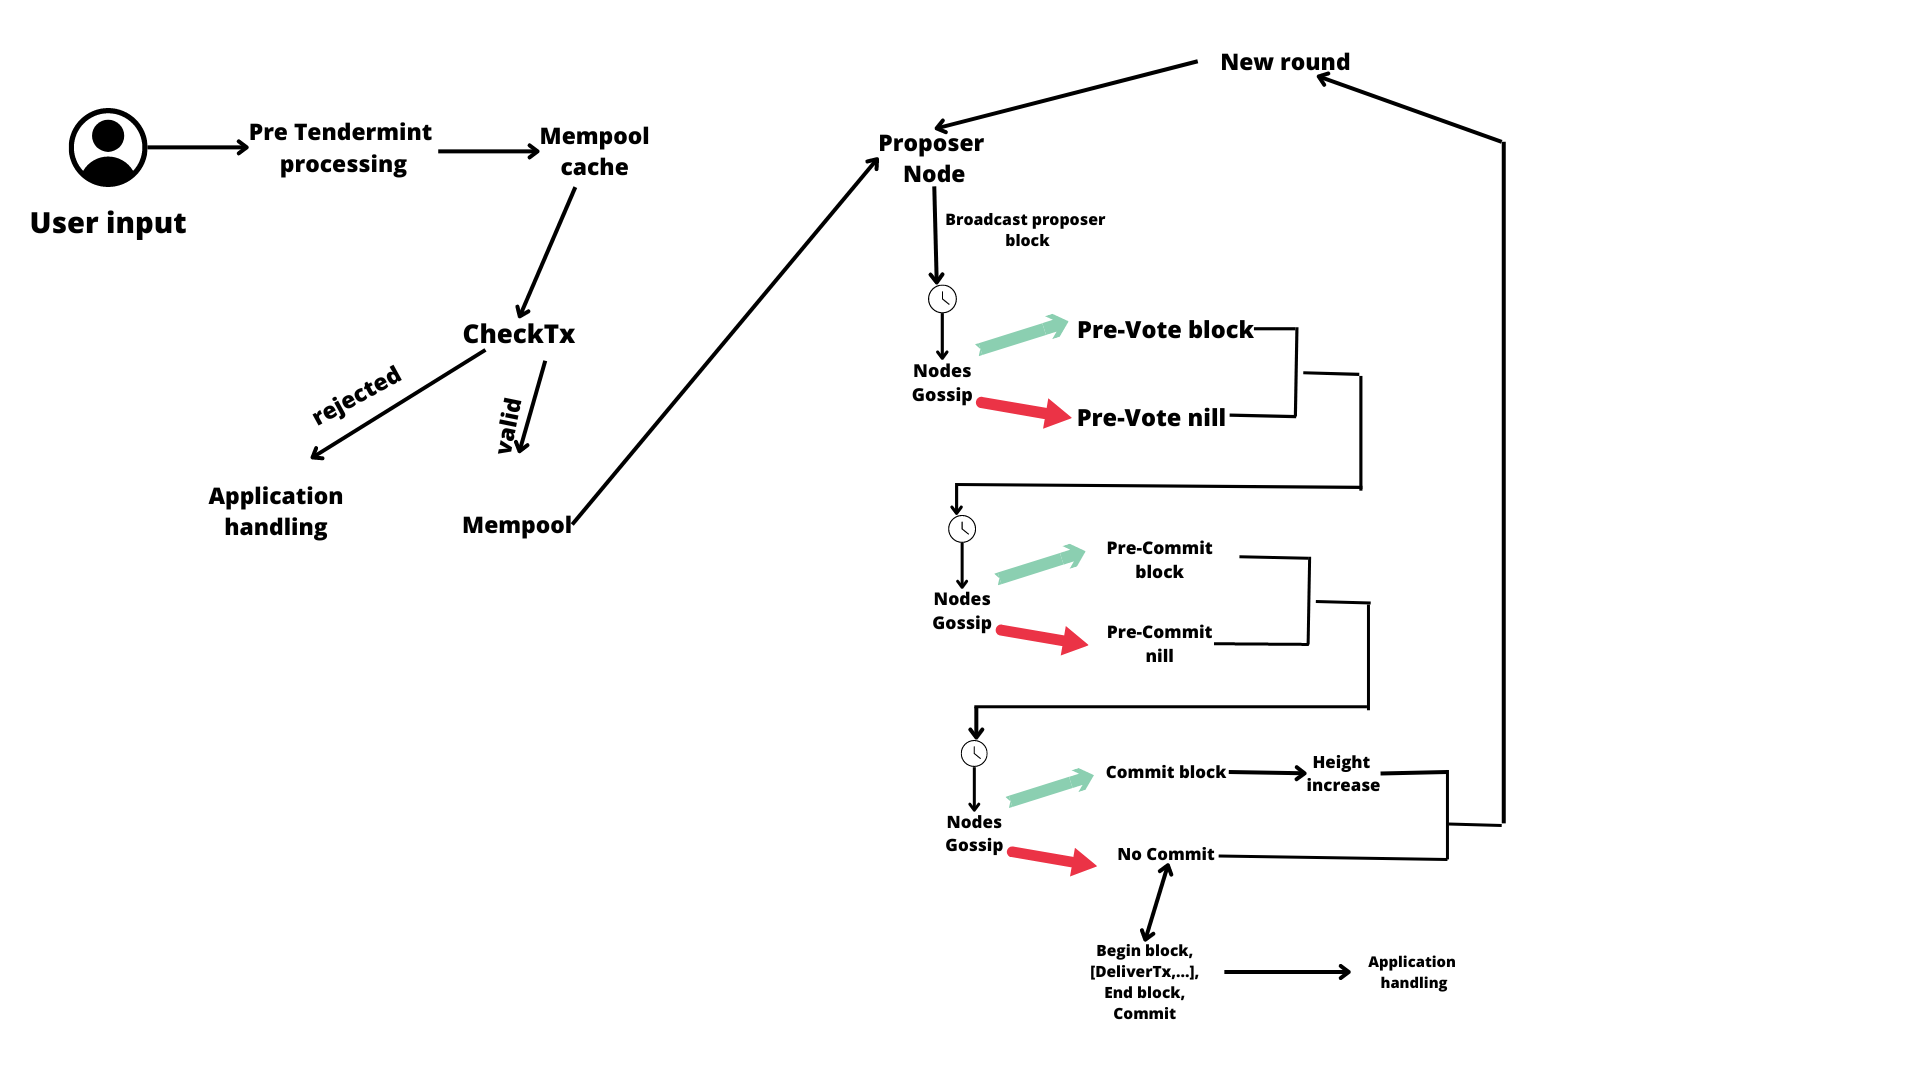
\includegraphics[width=1\textwidth]{Userinput} 
	\caption{Tendermint in a nutshell}
\end{figure}\\
\newpage
	\section{Experiments}
	\subsection{Implementation choices and potential limitations}
	At this point let's switch to experiments we did on Tendermint. First of all we discuss briefly the implementations choices. We did those experiments on Tendermint 0.34.24 version, using docker to simulate a network of validators that run the consensus algorithm. The operating system on which we have built our experiments is Ubuntu 22.04. This set up obviously is not ideal for testing a real system, since we have that all nodes run in a local machine, we can not simulate real network. Indeed in this scenario, links work at full speed continuously, never experiencing slowdown. Also we must consider the fact that the machines on which we did the experiments are laptops with limited computational power. Both of us are equipped with a 4 core processor, therefore we thaught that was not useful to do testing on networks composed by more than 4 validators nodes.
	\subsection{Functionality analysis}
	Once we set up Tendermint running with Docker, we started to test the basic functionalities. The ABCI implemented is a simple key-value store application, it simply stores in blocks transactions that are proposed by clients (in this case a simple command line through wich we submit transactions and query the blockchain to check if they are inserted). \\ \\ 
	First of all we start by checking the status of the application by inserting in a terminal the following command:
	\begin{lstlisting}[style=bashstyle]
	curl -s localhost:26657/status
	\end{lstlisting}
	when, the application is running it responds with a message in JSON format which includes a lot of information like: the protocol version, the address and port on which the application is running, latest blockchain height, latest blockchain time, hash of the last block and many others. \\
	We can also query the status of the chain and searching for specific field and not returning the whole status, in the following example we ask for $latest_app_hash$ in particular.
	\begin{lstlisting}[style=bashstyle]
	curl http://localhost:26657/status | json_pp | grep latest_app_hash	
	\end{lstlisting}
	When the key-value store app is running we can start sending transactions with the following command:
	\begin{lstlisting}[style=bashstyle]
	curl -s 'localhost:26657/broadcast_tx_commit?tx="abcd"'
	\end{lstlisting}
	When a transaction is sent to a Tendermint node, it will run via CheckTx against the application. If it passes CheckTx, it will be included in the mempool, broadcasted to other peers, and eventually included in a block.
	We can use the following command to check if the transaction reached the validators and is inserted in the block chain:
	\begin{lstlisting}[style=bashstyle]
	curl -s 'localhost:26657/abci_query?data="abcd"'
	\end{lstlisting}
	We can also decide to send transactions with a key value too:
	\begin{lstlisting}[style=bashstyle]
	curl -s 'localhost:26657/broadcast_tx_commit?tx="name=xxx"'
	\end{lstlisting}
	and then query the key to get back the value in hexadecimal format:
	\begin{lstlisting}[style=bashstyle]
	curl -s 'localhost:26657/abci_query?data="name"'
	\end{lstlisting}
	Everytime Tendermint starts, if a blockchain exists, it will take some time before starting for reading and loading all the existing blockchain. Once the blockchain is read Tendermint starts to run consensus and produce blocks. If we want to start a brand new chain and reset the old one, stop the nodes and run:
	\begin{lstlisting}[style=bashstyle]
	tendermint unsafe_reset_all
	\end{lstlisting}
	This command will remove the data directory and reset private validator and address book files.\\
\newline
	To start a testnet composed by 4 nodes (validators) we have to open a terminal, go to the path where Tendermint is and run the following commands:
	\begin{lstlisting}[style=bashstyle]
	make build-linux   
	make localnet-start 
	\end{lstlisting}
	at this point nodes are created and successfully running. The nodes bind their RPC servers to ports 26657, 26660, 26662, and 26664 on the host.
The nodes of the network expose their P2P and RPC endpoints to the host machine on ports 26656-26657, 26659-26660, 26661-26662, and 26663-26664 respectively
	\subsection{benchmarks}
	
	

	
	
\end{document}